\documentclass{beamer}
%\usecolortheme{spruce}
\usetheme{A}

\usepackage{amsmath}
\usepackage{datetime}
\usepackage{relsize}
\usepackage{ulem}
\usepackage{amsmath}
\usepackage{calc}
\usepackage{tikz}
\usepackage{tabularx}
\usepackage{stmaryrd}
\usepackage{wasysym}
\usepackage{booktabs}
\usepackage{multicol}
\usepackage{colortbl}

\definecolor{darkgreen}{HTML}{006400}
\definecolor{darkred}{HTML}{8b0000}
\newcommand{\dg}[1]{\textcolor{darkgreen}{#1}}
\newcommand{\dr}[1]{\textcolor{darkred}{#1}}
\newcommand{\happy}{\dg{\smiley}}
\newcommand{\sad}{\dr{\frownie}}

\newcolumntype{L}{>{\raggedright\arraybackslash}X}
\newcommand{\hnorm}{\vphantom{()}}

\hypersetup{
    colorlinks=true,
    urlcolor=blue,
    pdfpagemode=FullScreen,
}


\begin{document}



\date{CLIN 32, June 2022, Tilburg}

\title[]{Geometry-Aware Supertagging}
\subtitle[]{with Heterogeneous Dynamic Convolutions}
\author{%
    Konstantinos Kogkalidis \and \& \and Michael Moortgat\\ 
    \inst{Utrecht Institute of Linguistics OTS, Utrecht University}
}


{%
\setbeamertemplate{headline}{}
\frame{\titlepage
\hspace{-10pt}
\begin{minipage}{0.5\textwidth}
\begin{minipage}{0.35\textwidth}

\includegraphics[scale=0.065]{NWO logo - RGB_wit_rondom_0.jpg}%
\end{minipage}%
\begin{minipage}{0.65\textwidth}
\smaller[3]
\centering
A composition calculus for vector-based semantic modelling
with a localization for Dutch\\~\\
NWO 360-89-070, 2017-\alert{\textbf{2022} (!!!)}
\end{minipage}
\end{minipage}%
\hfill
\begin{minipage}{0.45\textwidth}
\hfill
\raisebox{-5.5pt}{
\includegraphics[scale=0.5]{UU_logo_2021_EN_RGB.jpg}}
\end{minipage}%
}
}


%{%
%\setbeamertemplate{headline}{}
%\begin{frame}{Overview}
%\begin{block}{\alert{tl;dr}}
%\begin{itemize}
%    \item Categorial Grammars \& Supertagging
%    \item A decoding order for (sequence-of-trees)-shaped topologies
%    \item Bigger numbers than previous biggest numbers
%\end{itemize}
%\end{block}
%\end{frame}
%}


\section{Categorial Grammars}

\begin{frame}{Categorial Grammars 101}
    \smaller
    \begin{block}{\textbf{\smaller what are they?}}
    A \textbf{family} of syntactic formalisms; each instance consists of:
        \begin{itemize}
            \item a \textbf{lexicon}\\
            a map assigning \textit{categories} to words:
            (quasi-)logical formulas (or ADTs)
            \item a small set of \textbf{inference rules}\\
            ways to combine and reduce \textit{expressions} based on their categories 
        \end{itemize}
    \end{block}
\end{frame}

\begin{frame}{Categorial Grammars 101}
    \smaller
    \textbf{Many variations}: TLG, ACG, CCG, \dots ({\text{*}}CG)\\
    \hfill
    
    \alt<2->{
        \begin{block}{\smaller \textbf{divergences}}
            different background logics $\implies$
            \begin{itemize}
                \item different linguistic aspects captured\\
                \textit{e.g. surface order, non-local syntax, dependency relations}
                \item different parsing complexity\\
                \item different computational semantics\\
                \item \dots
            \end{itemize}
        \end{block}
        \vfill
    }
    {
        \begin{block}{\smaller \textbf{common points}}
            \begin{itemize}
                \item \textbf{Lexicalized}\\
                words come packed with their combinatorics 
                \item \textbf{Formal}\\
                proximal to logics, type theory \& functional programming
                \item \textbf{Transparent}\\
                neat syntax-semantics interface
            \end{itemize}
        \end{block}
    }
\end{frame}

\begin{frame}{Categorial Grammars 101}
    \smaller
    
    \begin{block}{\smaller{\alert{but!} the \textbf{parsing pipeline} is always the same}}
    given an input sentence:
        \begin{enumerate}
            \item Assign a category to each word
            \item Build the syntactic derivation bottom-up
            \item ???
            \item Profit
        \end{enumerate}
    \end{block}\vfill
    
    \noindent
    \hfill\makebox[30pt][l]{%
      \raisebox{0pt}[60pt][0pt]{%
        \includegraphics[scale=0.2]{Screenshot 2022-05-30 at 20-21-00 Underpants Gnomes.png}}
    }
    
\end{frame}

\section{Supertagging}


\begin{frame}{Supertagging: the task}
    \smaller
    For some input sentence $w_1, \dots w_n$ find the category assignment $c_1, \dots c_n$ s.t.
        \[
            argmax_{(c_1, \dots c_n)}~ p(c_1, \dots c_n ~ | ~ w_1, \dots w_n)^*
        \]
        
    \vfill
    \visible<2->{
    \begin{flushright}
    \begin{minipage}{0.875\textwidth}
    \smaller
    \textsuperscript{\text{*}}\textit{In practice}:\\
    \textit{build the best statistical model possible given current technology and available data}
    \end{minipage}
    \end{flushright}
    }
\end{frame}

\begin{frame}{Supertagging, traditionally}
    \smaller
    $
    p(c_1, \dots c_n ~ | ~ w_1, \dots w_n) \approx
    $
    \begin{itemize}
        \uncover<2->{
        \item $\prod_i^n (c_i~|~w_i)$\\
        \quad \textit{co-occurrence-based statistical models (90s)}}
        \uncover<3->{
        \item $\prod_i^n (c_i~|~w_{i-\kappa} \dots w_{i+\kappa})$\\
        \quad \textit{window-based n-gram models (00s), feed-forward networks (early 10s)}}
        \uncover<4->{
        \item $\prod_i^n (c_i~|~w_1,\dots w_n)$\\
        \quad \textit{sequence encoders (mid 10s)}}
        \uncover<5->{
        \item $\prod_i^n (c_i~|~c_1, \dots c_{i-1}, w_1,\dots w_n)$\\ 
        \quad \textit{seq2seq (late 10s)}}
    \end{itemize}
    \vfill
    
    
    \alt<6->{
    \textbf{in sum}
    \begin{enumerate}
        \item[$\bullet$] domain generalization
        \item[$\bullet$] wider receptive field
        \pause
        \item[$\bullet$] what about the co-domain?
    \end{enumerate}
    }
    {
        \centering
        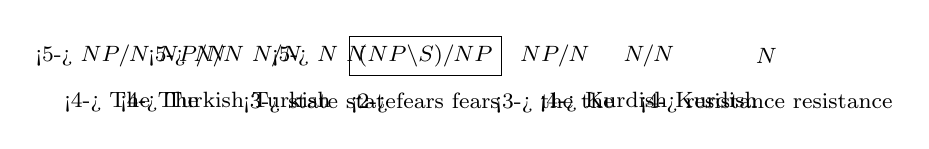
\begin{tikzpicture}
        \smaller
        %
        \node (the)         at (-8em, 0.06em)   {\alt<4->
                                                    {\alert{The}}
                                                    {The}
                                                };
        \node (t1)          at (-8em, 2em)      {\alt<5->
                                                    {\alert{$NP/N$}}
                                                    {$NP/N$}
                                                };
        %
        \node (turkish)     at (-4em, 0.06em)      {\alt<4->
                                                    {\alert{Turkish}}
                                                    {Turkish}
                                                };
        \node (t2)          at (-4em, 2em)      {\alt<5->
                                                    {\alert{$N/N$}}
                                                    {$N/N$}
                                                };
        %
        \node (state)       at (0em, 0em)       {\alt<3->
                                                    {\alert{state}}
                                                    {state}
                                                };
        \node (t3)          at (0em, 2em)       {\alt<5->
                                                    {\alert{$N$}}
                                                    {$N$}
                                                };
        %
        \node (fears)     at (4.5em, 0em)     {\alt<2->
                                                    {\alert{fears}}
                                                    {fears}
                                                };
        \node (t4)          at (4.5em, 2em)     {
                                                $\boxed{
                                                {(NP\backslash S)/NP}}$};
        %
        \node (the2)        at (10em, 0em)      {\alt<3->
                                                    {\alert{the}}
                                                    {the}
        
                                                 };
        \node (t5)          at (10em, 2em)       {$NP/N$};
        %
        \node (Kurdish)     at (14em, 0.03em)   {\alt<4->
                                                {\alert{Kurdish}}
                                                    {Kurdish}
                                                };
        \node (t6)          at (14em, 2em)      {$N/N$};
        %
        \node (resistance)  at (19em, 0em)   {\alt<4->
                                                    {\alert{resistance}}
                                                    {resistance}
                                                };
        \node (resistance)  at (19em, 2em)      {$N$}; 
        \end{tikzpicture}
    }
\end{frame}

\begin{frame}{Intermezzo: the curse(?) of sparsity}
    \smaller
    The majority of unique categories in common datasets are \alert{rare}
    \vfill

    \pause
    the ``\textit{fix}'': ignore rare categories
    \begin{itemize}
        \item small penalty in accuracy
        \item less so for coverage..
        \item meta: sparse grammars = bad
    \end{itemize}
    
    \vfill
    
    \pause
    the \textbf{fix}: decompose categories \& build them up during decoding
    \begin{itemize}
        \item[\textcolor{blue}{\lightning}] unlimited \sout{power} generalization
        \item meta: sparse grammars = ok
    \end{itemize}
\end{frame}

\begin{frame}{Supertagging, constructively}
    \smaller
    $
    p(\sigma_1, \dots \sigma_m ~ | ~ w_1, \dots w_n) \approx
    $
    \begin{itemize}
        \uncover<2-12, 16->{
        \item $\prod_i^m (\sigma_i~|~\sigma_1, \dots \sigma_{i-1}, w_1,\dots w_n)$\\ 
        \quad \textit{sequential constructive~(w/ Moortgat \& Deoskar, 2019)}}
        \uncover<13->{
        \item $\prod_i^m (\sigma_i~|~\mathrm{anc}(\sigma_i),  w_1,\dots w_n)$\\
        \quad \textit{tree-recursive (Prange et. al 2020)}}
    \end{itemize}
    \vfill
    
    \alt<16->{
        \textbf{in sum}\\
        \centering
        \begin{tabularx}{0.85\textwidth}{@{}L@{\qquad}c@{~}c@{\qquad}c@{~}c@{}}
        \textit{output structure} & \multicolumn{2}{c}{sequence-like}          & \multicolumn{2}{c}{tree-like}\\
        \toprule
        \textit{context}           & \happy & \dg{global}      & \sad & \dr{local}\\
        \textit{complexity}        & \sad   & \dr{quadratic}   & \happy & \dg{constant}\\
        \textit{treeness}     		& \sad  & \dr{implicit, learned} & \happy & \dg{explicit, captured}\\
        \textit{sequenceness}      & \sad & \dr{misaligned} & \sad & \dr{ignored}\\
        \end{tabularx}
    }
    {
        \centering
        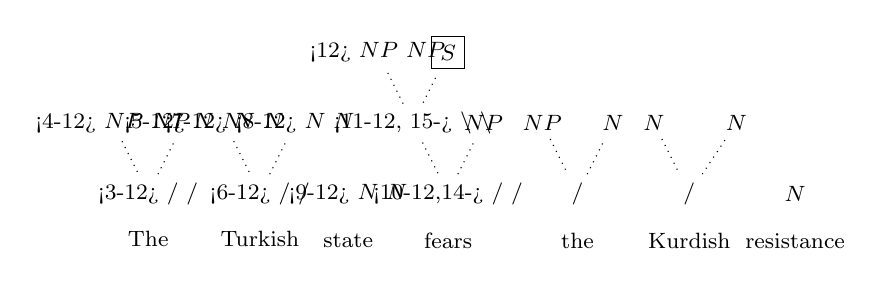
\begin{tikzpicture}
        \smaller
        %
        \node (the)         at (-8em,0.06em)    {\alert{The}};
        \node (t11)         at (-8em, 2em)      {\alt<3-12>
                                                    {\alert{$/$}}
                                                    {$/$}
                                                };
        \node (t12)         at (-9.5em, 5em)    {\alt<4-12>
                                                    {\alert{$NP$}}
                                                    {$NP$}
                                                };
        \node (t13)         at (-6.5em, 5em)    {\alt<5-12>
                                                    {\alert{$N$}}
                                                    {$N$}
                                                };
        \draw[dotted] (t12) -- (t11) -- (t13);
        %
        \node (turkish)     at (-3.25em,0.06em) {\alert{Turkish}};
        \node (t21)         at (-3.25em,2em)    {\alt<6-12>
                                                    {\alert{$/$}}
                                                    {$/$}
                                                };
        \node (t22)         at (-4.75em, 5em)   {\alt<7-12>
                                                        {\alert{$N$}}
                                                        {$N$}
                                                    };
        \node (t23)         at (-1.75em, 5em)   {\alt<8-12>
                                                    {\alert{$N$}}
                                                    {$N$}
                                                };
        \draw[dotted] (t22) -- (t21) -- (t23);
        %
        \node (state)       at (0.5em, 0em)     {\alert{state}};
        \node (t3)          at (0.5em, 2em)     {\alt<9-12>
                                                    {\alert{$N$}}
                                                    {$N$}
                                                };
        %
        \node (fears)     at (4.75em, 0em)    {\alert{fears}};
        \node (t41)         at (4.75em, 2em)    {\alt<10-12,14->
                                                    {\alert{$/$}}
                                                    {$/$}
                                                };
        \node (t42)         at (3.25em, 5em)    {\alt<11-12, 15->
                                                    {\alert{$\backslash$}}
                                                    {$\backslash$}
                                                };
        \node (t43)         at (6.25em, 5em)    {$NP$};
        \node (t44)         at (1.75em, 8em)    {\alt<12>
                                                    {\alert{$NP$}}
                                                    {$NP$}
                                                };
        \node (t45)         at (4.75em, 8em)    {$\boxed{S}$};
        \draw[dotted] (t45) -- (t42) -- (t44);
        \draw[dotted] (t42) -- (t41) -- (t43);
        %
        \node (the2)        at (10.25em, 0em)   {\alert{the}};
        \node (t51)         at (10.25em, 2em)   {$/$};
        \node (t52)         at (8.75em, 5em)    {$NP$};
        \node (t53)         at (11.75em, 5em)   {$N$};
        \draw[dotted] (t52) -- (t51) -- (t53);
        %
        \node (Kurdish)     at (15em, 0em)   {\alert{Kurdish}};
        \node (t61)         at (15em, 2em)      {$/$};
        \node (t62)         at (13.5em, 5em)    {$N$};
        \node (t63)         at (17em, 5em)      {$N$};
        \draw[dotted] (t62) -- (t61) -- (t63);
        %
        \node (resistance)      at (19.5em, 0em)    {\alert{resistance}};
        \node (resistance)      at (19.5em, 2em)    {$N$}; 
        \end{tikzpicture}
    }
\end{frame}

\section{Geometry}

\begin{frame}{A fresh perspective}
    \smaller
    neither sequence nor tree but \alert{sequence of trees}
    
    \pause
    $
    p(\sigma_1, \dots \sigma_m ~ | ~ w_1, \dots w_n) \approx \prod_i^m (\sigma_i~|~\sigma_j : \mathrm{depth}(\sigma_j) < \mathrm{depth}(\sigma_i), w_1,\dots w_n)$\\
    \vfill
    
    \centering
    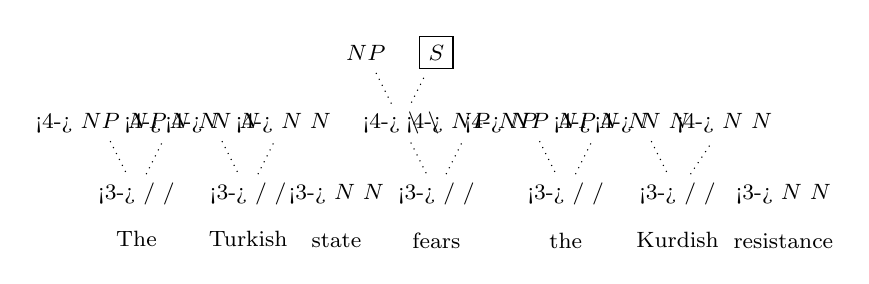
\begin{tikzpicture}
        \smaller
        %
        \node (the)         at (-8em,0.06em)    {\alert{The}};
        \node (t11)         at (-8em, 2em)      {\alt<3->
                                                    {\alert{$/$}}
                                                    {$/$}
                                                };
        \node (t12)         at (-9.5em, 5em)    {\alt<4->
                                                    {\alert{$NP$}}
                                                    {$NP$}
                                                };
        \node (t13)         at (-6.5em, 5em)    {\alt<4->
                                                    {\alert{$N$}}
                                                    {$N$}
                                                };
        \draw[dotted] (t12) -- (t11) -- (t13);
        %
        \node (turkish)     at (-3.25em,0.06em) {\alert{Turkish}};
        \node (t21)         at (-3.25em,2em)    {\alt<3->
                                                    {\alert{$/$}}
                                                    {$/$}
                                                };
        \node (t22)         at (-4.75em, 5em)   {\alt<4->
                                                        {\alert{$N$}}
                                                        {$N$}
                                                    };
        \node (t23)         at (-1.75em, 5em)   {\alt<4->
                                                    {\alert{$N$}}
                                                    {$N$}
                                                };
        \draw[dotted] (t22) -- (t21) -- (t23);
        %
        \node (state)       at (0.5em, 0em)     {\alert{state}};
        \node (t3)          at (0.5em, 2em)     {\alt<3->
                                                    {\alert{$N$}}
                                                    {$N$}
                                                };
        %
        \node (fears)     at (4.75em, 0em)    {\alert{fears}};
        \node (t41)         at (4.75em, 2em)    {\alt<3->
                                                    {\alert{$/$}}
                                                    {$/$}
                                                };
        \node (t42)         at (3.25em, 5em)    {\alt<4->
                                                    {\alert{$\backslash$}}
                                                    {$\backslash$}
                                                };
        \node (t43)         at (6.25em, 5em)    {\alt<4->
                                                    {\alert{$NP$}}
                                                    {$NP$}
                                                };
        \node (t44)         at (1.75em, 8em)    {$NP$};
        \node (t45)         at (4.75em, 8em)    {$\boxed{S}$};
        \draw[dotted] (t45) -- (t42) -- (t44);
        \draw[dotted] (t42) -- (t41) -- (t43);
        %
        \node (the2)        at (10.25em, 0em)   {\alert{the}};
        \node (t51)         at (10.25em, 2em)   {\alt<3->
                                                    {\alert{$/$}}
                                                    {$/$}
                                                };
        \node (t52)         at (8.75em, 5em)    {\alt<4->
                                                    {\alert{$NP$}}
                                                    {$NP$}
                                                };
        \node (t53)         at (11.75em, 5em)   {\alt<4->
                                                    {\alert{$N$}}
                                                    {$N$}
                                                };
        \draw[dotted] (t52) -- (t51) -- (t53);
        %
        \node (Kurdish)     at (15em, 0.03em)   {\alert{Kurdish}};
        \node (t61)         at (15em, 2em)      {\alt<3->
                                                    {\alert{$/$}}
                                                    {$/$}
                                                };
        \node (t62)         at (13.5em, 5em)    {\alt<4->
                                                    {\alert{$N$}}
                                                    {$N$}
                                                };
        \node (t63)         at (17em, 5em)      {\alt<4->
                                                    {\alert{$N$}}
                                                    {$N$}
                                                };
        \draw[dotted] (t62) -- (t61) -- (t63);
        %
        \node (resistance)      at (19.5em, 0em)    {\alert{resistance}};
        \node (resistance)      at (19.5em, 2em)    {\alt<3->
                                                    {\alert{$N$}}
                                                    {$N$}
                                                };
    \end{tikzpicture}
\end{frame}

\begin{frame}{Implementation: dynamic graph convolutions}
    \smaller 
    1 decoding step per tree depth; 3 message-passing rounds per step
    \begin{itemize}
        \item \textit{contextualize: states $\to$ states}\\
        \quad \alert{universal transformer encoder w/ relative weights}\\
        \quad (many-to-many, update states with neighborhood context)
        \item \textit{predict: state $\to$ nodes}\\
        \quad \alert{token classification w/ dynamic tree embeddings}\\
        \quad (one-to-many, predict fringe nodes from current state)
        \item \textit{feedback: nodes $\to$ state}\\
        \quad \alert{heterogeneous graph attention}\\
        \quad (many-to-one, update state with last predicted nodes)
    \end{itemize}
\end{frame}

\begin{frame}{Table with numbers}
        \vspace{-10pt}
        \smaller[2]
        \centering
        \begin{tabularx}{0.99\textwidth}{@{}l@{~}L@{}c@{\quad}c@{\quad}c@{\quad}c@{\quad}c@{}}
        & & \multicolumn{5}{c}{\textbf{accuracy} {(\%)}} \\
        \cmidrule(lr){3-7}
        & \multicolumn{1}{c}{\textbf{model}} & {overall} & {frequent} & {uncommon} & {~~rare~~} & {unseen}\\
        \toprule
        \multicolumn{7}{c}{\textit{\textbf{CCGbank} (Combinatory Categorial Grammar, en)}} \\
        \rowcolor{gray!20}
        & Sequential RNN            & 95.10 & 95.48 & 65.76 & 26.02 & 0.00\\
        & Tree Recursive            & 96.09 & 96.44 & 68.10 & \fbox{37.40} & 3.03\\
        % & BERT baseline             & 96.22 & 96.58 & 70.29 & 23.17 & -- \\
        \rowcolor{gray!20}
        & Attentive Convolutions    & 96.25 & \fbox{96.64} & 71.04 & --   & -- \\
        & \textit{this work}         & \fbox{96.29} & 96.61 & \fbox{72.06} & 34.45 & \fbox{4.55}\\
        \addlinespace
        \multicolumn{7}{c}{\textit{\textbf{CCGrebank} (ditto, improved version)}}\\
        \rowcolor{gray!20}
        & Sequential RNN            & 94.44 & 94.93 & 66.90 & 27.41 & 1.23\\
        & Tree Recursive            & 94.70 & 95.11 & 68.86 & 36.76 & \fbox{4.94}\\
        % & BERT baseline             & 94.83 & 95.27 & 68.86 & 23.99 & --\\
        \rowcolor{gray!20}
        & \textit{this work}        & \fbox{95.07} & \fbox{95.45} & \fbox{71.40} & \fbox{37.19} & 3.70\\
        \addlinespace
        \multicolumn{7}{c}{\textit{\textbf{TLGBank} (Lambek calculus \& control modalities, fr)}}\\
        \rowcolor{gray!20}
        & ELMo LSTM                 & 93.20 & 95.10 & 75.19 & 25.85 & -- \\
        % & BERT baseline             & \fbox{95.93} & \fbox{96.44} & 81.39 & 47.45 & --\\
        % \rowcolor{gray!20}
        & \textit{this work}        & \fbox{95.93} & \fbox{96.40} & \fbox{81.48} & \fbox{55.37} & \fbox{7.26}\\
        \addlinespace
        \multicolumn{7}{c}{\textit{\textbf{\AE thel} (van Benthem calculus \& dependency modalities, nl)}}\\
        \rowcolor{gray!20}
        & Sequential Transformer      & 83.67 & 84.55 & 64.70 & 50.58 & \fbox{24.55}\\
        % & BERT baseline             & 93.52 & \fbox{94.83} & 71.85 & 38.06 & --\\
        % \rowcolor{gray!20}
        & \textit{this work}        & \fbox{93.67} & \fbox{94.72} & \fbox{73.45} & \fbox{53.83} & 15.78\\
        \end{tabularx}
\end{frame}

\begin{frame}{What of it}
    \smaller 
    \alert{model}
    \begin{itemize}
    	\item[\happy] \dg{global context}
    	\item[\happy] \dg{constant decoding}
    	\item[\happy] \dg{input/output alignment}
    	\item[\happy] \dg{explicit tree structures}
    \end{itemize}
    \vfill
    
    \pause
    \alert{sparsity}.. a \textit{friend}?
    \begin{itemize}
        \item more rare cats $\implies$ better acquisition of rare cats
        \item cascading effect on performance
    \end{itemize}
    \vfill
    
    \pause
    \alert{todo}
    \begin{itemize}
        \item beam search: open problem
        \item parser integration
    \end{itemize}
\end{frame}

{\setbeamertemplate{headline}{}
\frame{

\begin{center}
    thanks!    
\end{center}

\smaller

\vfill

    \textit{arXiv} \hfill(includes: mathy equations, more and bigger tables!) \\
    \href{https://arxiv.org/abs/2203.12235}{abs/2203.12235}
    \\[2\baselineskip]
    \textit{github} \hfill(includes: mostly working code! be the first to star!) \\
    \href{https://github.com/konstantinosKokos/dynamic-graph-supertagging}{konstantinosKokos/dynamic-graph-supertagging}
\vfill

\centering
\textbf{\alert{Boycott EMNLP'22}}
}

}


\end{document}